\documentclass{standalone}
\usepackage{pdfpages}
\usepackage{tikz}
\usepackage{amssymb}

\usetikzlibrary{shapes, chains, arrows, fit, calc, arrows.meta}
\tikzset{>={Stealth[width=3mm,length=3mm]}}

\newcommand{\mb} {\mathbf}
\def \minnodewidth {4.5cm}
\def \minrad {4cm}

%%%%%%%%%%%%%%%%%%%%%%%%%%%%%%%%%%%%%%%%%%%%%%%%%%%%%%%%%%%%%%%%%%%%%%%%%%%%%%%%

\begin{document}

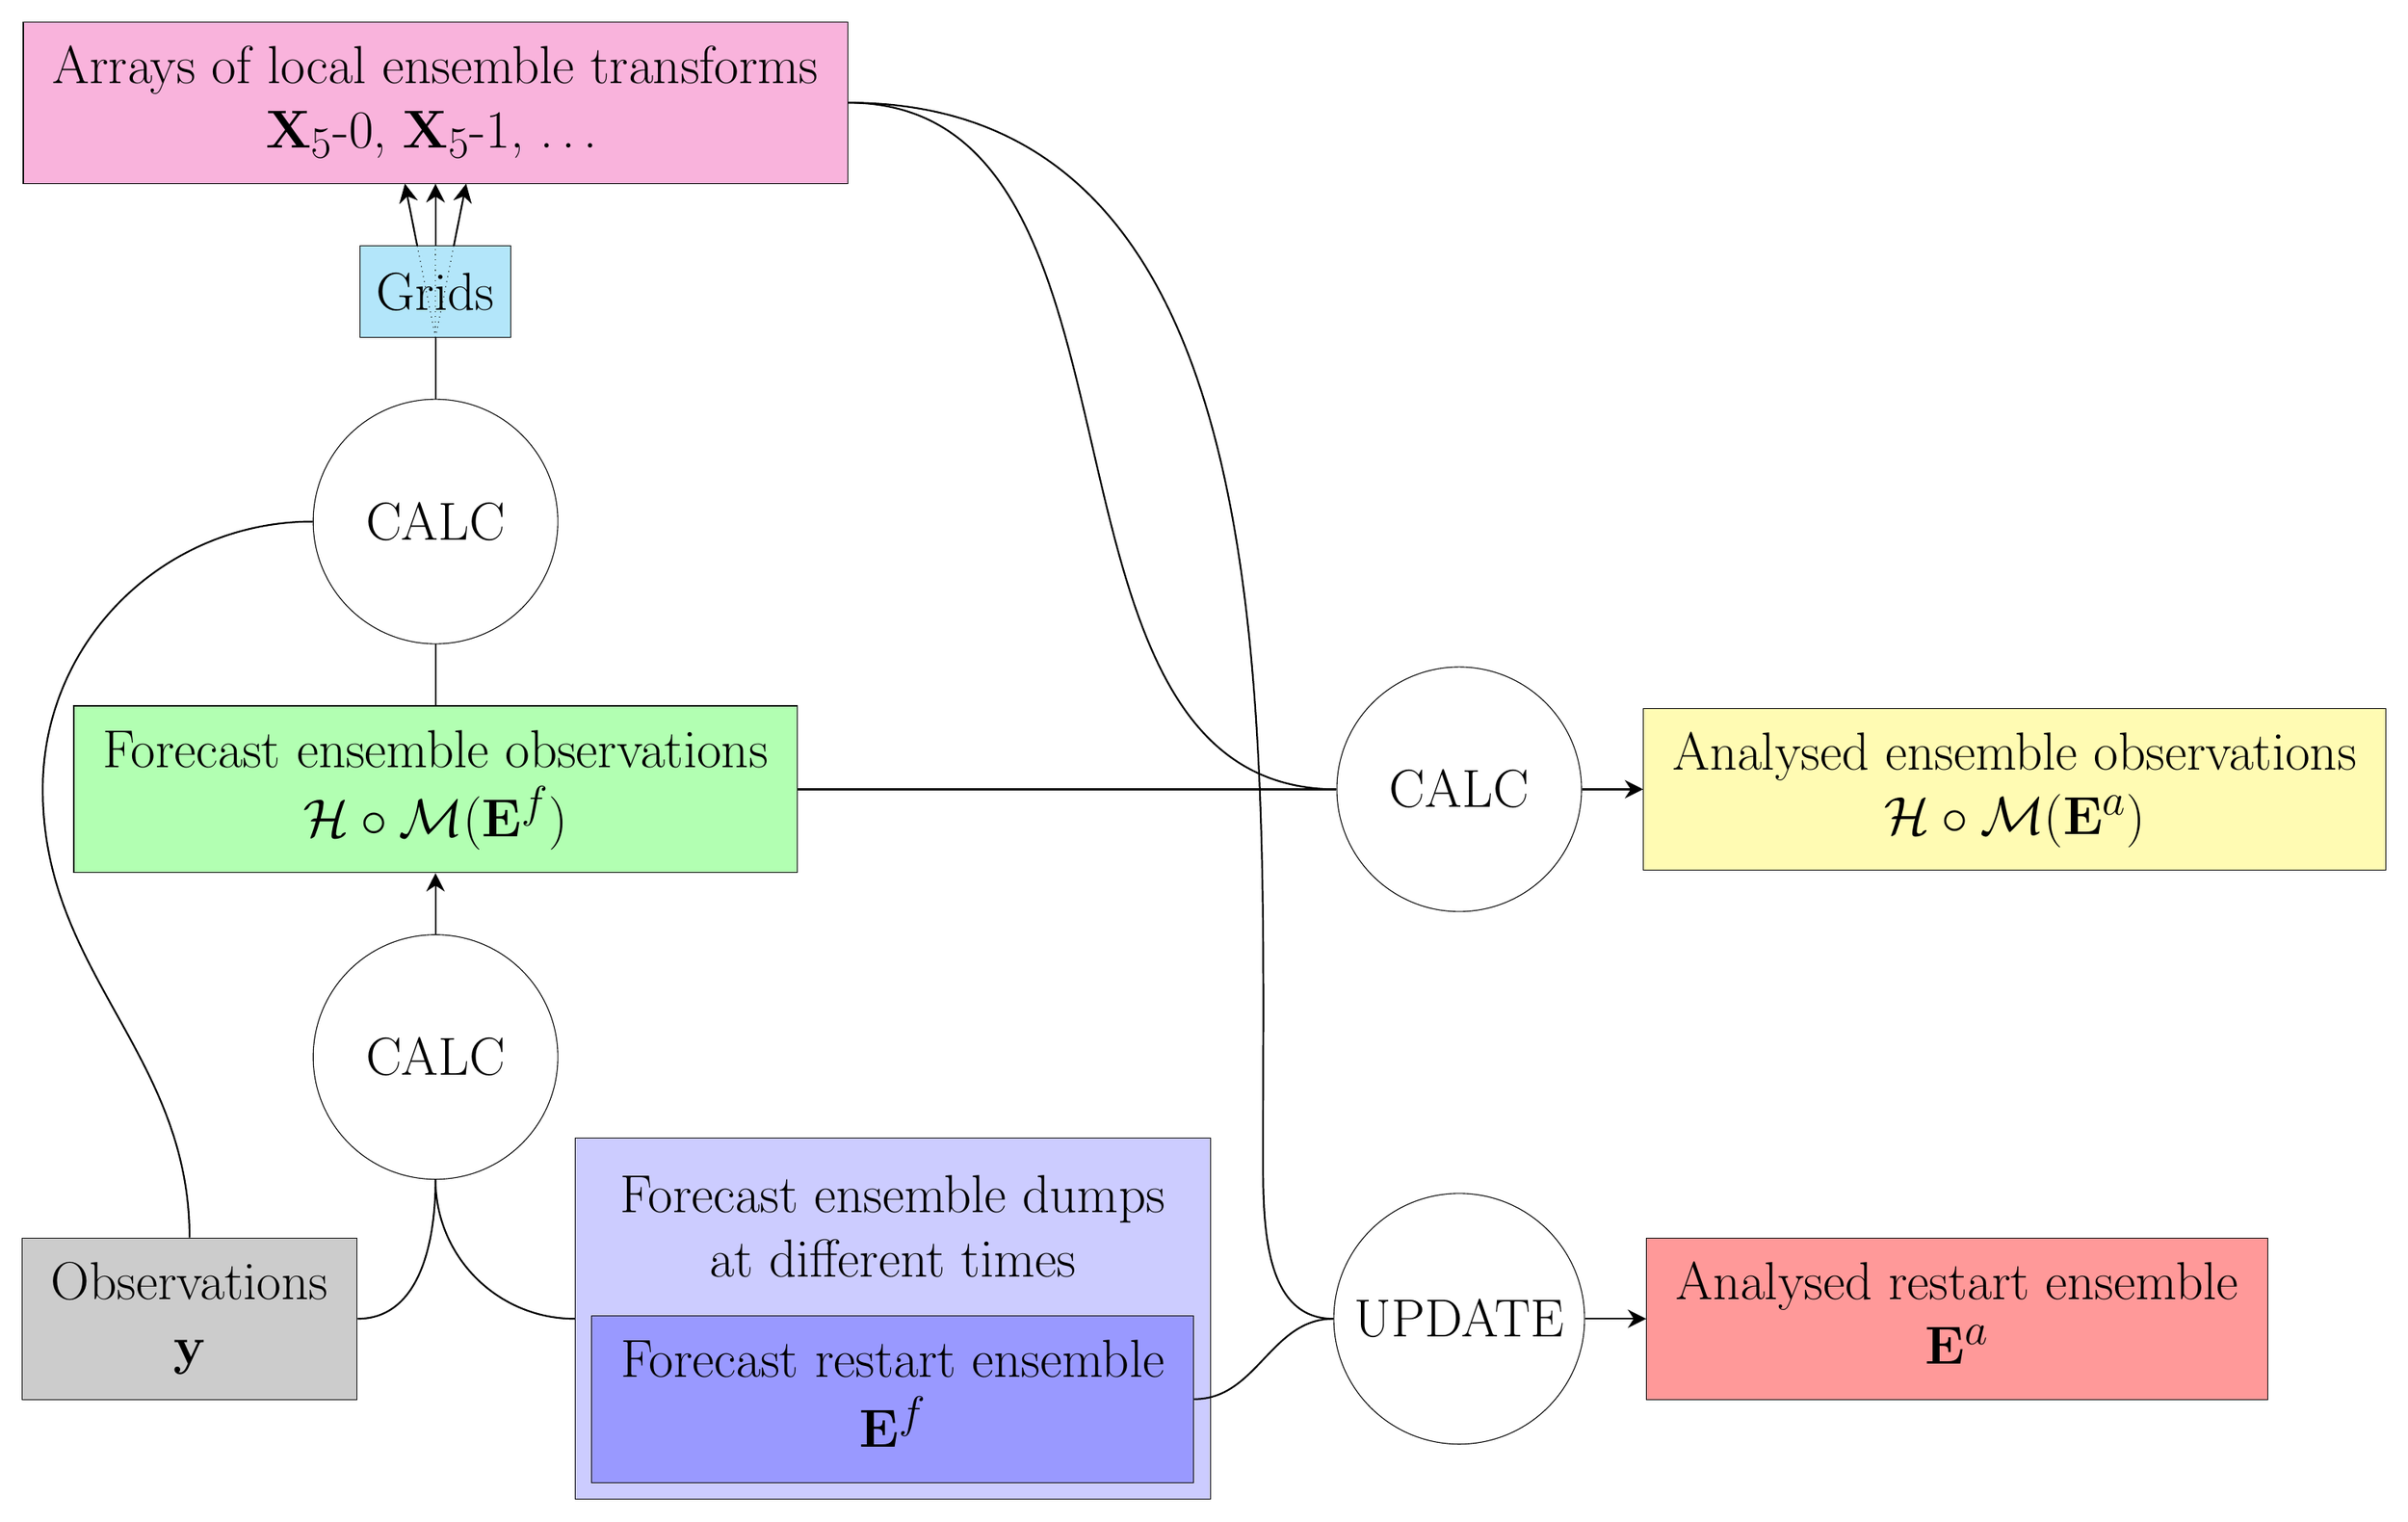
\begin{tikzpicture}
\Huge

\node (frens) [transparent, draw, minimum width = \minnodewidth] {\begin{tabular}{c}Forecast restart ensemble\\$\mb E^f$\end{tabular}};
\node (fensd) [transform shape, draw, fill = blue!20, fit = {(frens) ($(frens.center) + (0, 40mm)$)}, minimum width = \minnodewidth] {\begin{tabular}{c}Forecast ensemble dumps\\ at different times\\ \\\end{tabular}};
\node (frens) [draw, fill = blue!40, minimum width = \minnodewidth] {\begin{tabular}{c}Forecast restart ensemble\\$\mb E^f$\end{tabular}};
\node (origin) [transparent, left = 2cm of fensd] {};
\node (obs) [draw, fill = gray!40, left = of origin, minimum width = \minnodewidth] {\begin{tabular}{c}Observations\\$\mb y$\end{tabular}};
\node (add1) [circle, draw, minimum width = \minrad, above = 2cm of origin] {CALC};
\node (ensobs) [draw, fill = green!30, above = 1cm of add1, minimum width = \minnodewidth] {\begin{tabular}{c} Forecast ensemble observations\\$\mathcal H \circ \mathcal M (\mb E^f)$\end{tabular}};

\draw[-, thick] (obs) to [in = -90, out = 0] (add1.south);
\draw[-, thick] (fensd) to [in = -90, out = 180] (add1.south);
\draw[-, thick] (add1.south) to (add1);
\draw[->, thick] (add1) to (ensobs);

\node (add21) [circle, transparent, minimum width = \minrad, above = 1cm of ensobs] {CALC};
\node (grids) [transparent, above = 1cm of add21, minimum width = 1.5cm, minimum height = 1.5cm] {Grids};

\node (transforms) [draw, fill = magenta!30, above = 1cm of grids, minimum width = \minnodewidth] {\begin{tabular}{c}Arrays of local ensemble transforms\\$\mb X_5$-0, $\mb X_5$-1, \dots \end{tabular}};

\draw[-, thick] (ensobs) to (grids.south);
\draw[->, thick] (grids.south) to ([out = 90, in = 90, xshift = -5mm] transforms.south);
\draw[->, thick] (grids.south) to ([out = 90, in = 90] transforms.south);
\draw[->, thick] (grids.south) to ([out = 90, in = 90, xshift = 5mm] transforms.south);
\node (grids) [draw, fill = cyan!30, above = 1cm of add21, minimum width = 1.5cm, minimum height = 1.5cm] {Grids};
\draw[->, dotted] (grids.south) to ([out = 90, in = 90, xshift = -5mm] transforms.south);
\draw[->, dotted] (grids.south) to ([out = 90, in = 90] transforms.south);
\draw[->, dotted] (grids.south) to ([out = 90, in = 90, xshift = 5mm] transforms.south);
\node (add21) [circle, draw, fill = white, minimum width = \minrad, above = 1cm of ensobs] {CALC};
\draw[-, thick] (obs) to [out = 90, in = -90] ([xshift = -0.5cm] ensobs.west) to [out = 90, in = 180] (add21);

\node (add2) [circle, draw, minimum width = \minrad, right = 2cm of fensd] {UPDATE};
\draw[-, thick] (frens.east) to [out = 0, in = 180] (add2.west);

\node (arens) [draw, fill = red!40, minimum width = \minnodewidth, right = 1cm of add2] {\begin{tabular}{c}Analysed restart ensemble\\$\mb E^a$\end{tabular}};
\draw[->, thick] (add2) to (arens);

\node (add3) [circle, draw, minimum width = \minrad] at (ensobs -| add2) {CALC};
\draw[-, thick] (transforms.east) to [out = 0, in = 180] (add3.west);
\draw[-, thick] (ensobs.east) to [out = 0, in = 180] (add3.west);

\node (aensobs) [draw, fill = yellow!30, right = 1cm of add3, minimum width = \minnodewidth] {\begin{tabular}{c} Analysed ensemble observations\\$\mathcal H \circ \mathcal M (\mb E^a)$\end{tabular}};
\draw[->, thick] (add3) to (aensobs);

\draw[-, thick] (transforms.east) to [out = 0, in = 90] ([xshift = -1.2cm, yshift = -6cm] add3.west) to [out = -90, in = 180] (add2.west);

\end{tikzpicture}
\end{document}
